\documentclass{beamer}
\usepackage{tikz}
\usetikzlibrary{arrows,positioning,decorations.pathmorphing,decorations.markings}
\tikzstyle{vecArrow} = [thick, decoration={markings,mark=at position 1 with {\arrow[semithick]{open triangle 60}}}, double distance=1.4pt, shorten >= 5.5pt, preaction = {decorate}, postaction = {draw,line width=1.4pt,white,shorten >= 4.5pt}]
\tikzstyle{innerWhite} = [semithick,white,line width=1.4pt,shorten >= 4.5pt]
\usepackage{bookman}
\usetheme{Berlin}
\usecolortheme{beaver}

\title{Understanding the imprinting mechanism of \textit{Ube3a} for therapeutic intervention}
\author{Jade M. Benjamin}
\institute[TAMU]{
  Texas A\&M University
  \and
  Department of Veterinary Pathobiology\\
  Interdisciplinary Genetics Program
}
\date{October 14th, 2016}
%% \logo{\includegraphics[height=1.5cm]{tamu-logo.pdf}}
%% \AtBeginSection[]{
%%   \begin{frame}
%%     \frametitle{Outline}
%%     \tableofcontents[currentsection]
%%   \end{frame}
%% }

\begin{document}

\frame{\titlepage}

\section{Introduction}

\begin{frame}
  \resizebox{\linewidth}{!}{
    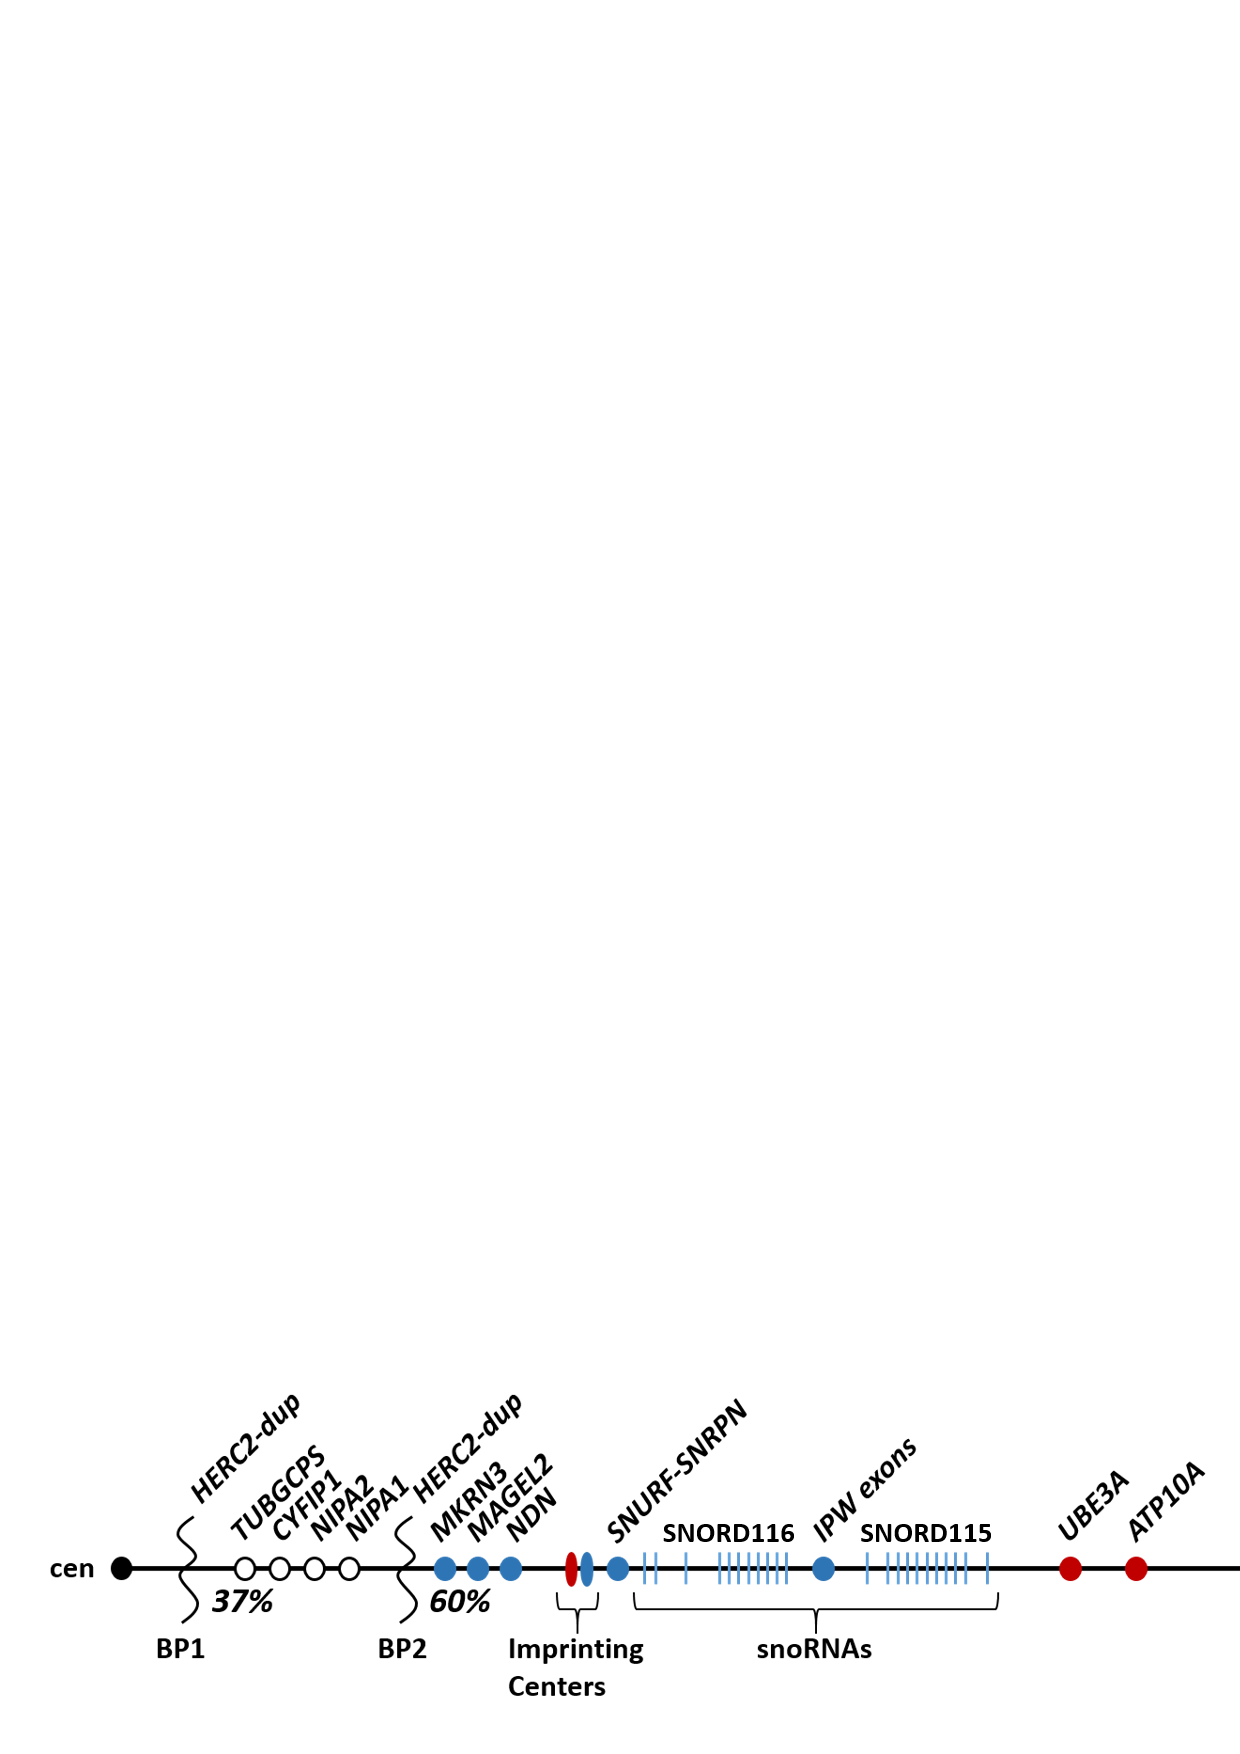
\includegraphics{figures/15q11-q13_region2.pdf}
  }

  \begin{block}{\textbf{Figure 1.1}}
  The frequent rearrangements of human chromosome 15q11-q13 region is due to recombination hotspots of the \textit{HERC2} duplicons at the three breakpoints (BP). Paternally expressed genes in blue, maternally expressed genes in red, and biallelically expressed genes in white.
  \end{block}
\end{frame}

\begin{frame}
  \resizebox{\linewidth}{!}{
    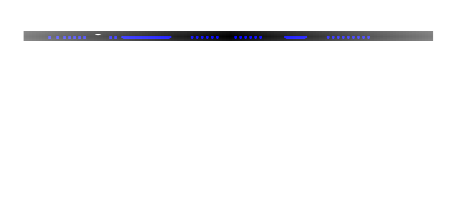
\includegraphics{figures/paternal-transcription2.pdf}
  }
  
  \begin{block}{\textbf{Figure 1.2}}
  Paternal expression of long alternatively spliced transcript in neurons comprising \textit{SNURF/SNRPN}, C/D box snoRNAs (\textit{SNORD116} and \textit{SNORD115}), \textit{IPW}, and \textit{UBE3A-AS} is controlled by unmethylated Prader-Willi syndrome imprinting center region (ICR). There some unknown mechanism \textit{UBE3A-AS} inhibits expression of paternal \textit{UBE3A}. Paternally expressed genes in blue and paternally silenced \textit{UBE3A} in black.
  \end{block}
\end{frame}

\begin{frame}
  \resizebox{\linewidth}{!}{
    \includegraphics{figures/Genomic-Imprinting-Expression2.pdf}
  }

  \begin{block}{\textbf{Figure 1.3}}
  The majority of genes show biallelic expression with maternal (red) and paternal (blue) alleles expressed in all tissues. In a subset of genes via some epigenetic mechanism such as DNA methylation, gene expression is limited to monoallelic expression.
  \end{block}
\end{frame}

\begin{frame}
  \resizebox{\linewidth}{!}{
    \includegraphics{figures/lncRNAs2.pdf}
  }
  \begin{block}{\textbf{Figure 1.4}}
    Schematic of lncRNAs based on loci-of-origin depicting an enhancer RNA, sense and antisense overlapping RNAs, and an intergenic RNA.
  \end{block}
\end{frame}

\begin{frame}
  \begin{columns}
    \column{0.5\textwidth}
    %% \resizebox{\linewidth}{4cm}{
    \includegraphics[scale=0.50]{figures/FGFR2-AS2.pdf}
    %% }

    \column{0.5\textwidth}
    \begin{block}{\textbf{Figure 1.5}}
      \emph{FGFR2-AS} plays a central role in tissue-specific alternative splicing of \emph{FGFR2} via chromatin remodeling. The \emph{FGFR2} antisense transcript recruits PRC2 and KDM2a, which interfere with PTB repression of exon IIIb, resulting in exclusion of exon IIIc. PolII, polymerase II, antisense in red and sense strand in blue.
    \end{block}
  \end{columns}
  
\end{frame}

\begin{frame}
  \resizebox{\linewidth}{!}{
    \includegraphics[scale=0.45]{figures/AIRN2.pdf}
  }

    \textbf{Figure 1.6}
      Transcription of \emph{AIRN} regulates transcriptional gene silencing of the \emph{IGF2R} gene cluster. Continuous \emph{AIRN} transcription silences \emph{IGF2R} by transcriptional overlap of \emph{IGF2R} promoter. By some unknown mechanism, the \emph{IGF2R} promoter is irreversibly methylated. Silencing of \emph{SLC22A2} and \emph{SLC22A3} occurs through \emph{AIRN}-mediated recruitment of chromatin modifiers to their promoters. Maternal allele (red), paternal allele (blue), silenced genes (gray), and non-imprinting genes (white). Arrows denote direction of transcription.

\end{frame}

\begin{frame}
  \resizebox{\linewidth}{!}{
    \includegraphics[scale=0.44]{figures/Nespas2.pdf}
  }
  
  \begin{block}{\textbf{Figure 1.7}}
    \emph{Nespas} overlapping transcription occludes the \emph{Nesp} promoter, promoting CpG methylation silencing paternal expression of \emph{Nesp}. Maternal allele (red), paternal allele (blue), silenced genes (gray). Arrows denote direction of transcription. Zoom view of overlapping exons of \emph{Nesp} and \emph{Nespas}.
  \end{block}
\end{frame}

\begin{frame}
  \resizebox{\linewidth}{!}{
    \includegraphics[scale=1]{figures/NUDT6.pdf}
  }
  \begin{block}{\textbf{Figure 1.8}}
    The partial overlap of \emph{FGF-2} by the protein-coding gene \emph{NUDT6} regulates \emph{FGF-2} expression by forming double-stranded RNA duplexes reducing stability and translation efficiency. Arrows denote direction of transcription.
  \end{block}
\end{frame}

\begin{frame}
  \begin{columns}
    \column{0.5\textwidth}
    \resizebox{\textwidth}{!}{
      \includegraphics{figures/KCNQ1OT1.pdf}
    }
    
    \column{0.5\textwidth}
    \begin{block}{\textbf{Figure 1.9}}
      Long range silencing of the \emph{KCNQ1} imprinting gene cluster is due to \emph{KCNQ1OT1}. It is proposed that processing of \emph{KCNQ1OT1} results in small regulatory RNAs, which interact with the imprinted genes causing silencing. Maternal allele (red), paternal allele (blue), silenced genes (gray), and non-imprinted genes (white). Arrows denote the direction of transcription.
    \end{block}
  \end{columns}
  
\end{frame}

\begin{frame}
  \resizebox{\linewidth}{!}{
    \includegraphics[scale=1]{figures/BACE1-AS.pdf}
  }
  \begin{block}{\textbf{Figure 1.10}}
    \emph{BACE1-AS} increases stability of \emph{BACE1} via dsRNA duplexes. This increase in \emph{BACE1} stability results in increased protein levels of BACE1 creating a post-translational feed forward loop. Arrows denote the direction of transcription.
  \end{block}
\end{frame}


\begin{frame}
  \resizebox{\linewidth}{!}{
    \includegraphics[scale=1]{figures/BDNF.pdf}
  }
  \begin{block}{\textbf{Figure 1.11}}
    \emph{BDNF-AS} regulates \emph{BDNF} gene expression by forming double-stranded RNA resulting in the recruitment of chromatin modeling factors to the promoter of \emph{BDNF}. Arrow denotes the direction of transcription.
  \end{block}
\end{frame}

\begin{frame}
  \begin{columns}
    \column{0.5\textwidth}
    \resizebox{\textwidth}{!}{
      \includegraphics[scale=1]{figures/Ube3a-AS_mechanism.pdf}
    }

    \column{0.5\textwidth}
    \begin{block}{\textbf{Figure 1.12}}
      \emph{UBE3A-AS} regulates paternal \emph{UBE3A} expression in neurons. \textbf{A)} Transcriptional collision model for \emph{UBE3A-AS} regulation of \emph{UBE3A}. \textbf{B)} Purposed alternative splicing model for \emph{UBE3A-AS} regulation of \emph{UBE3A}. Polymerase II (Pol II), antisense Pol II in red and sense Pol II in blue. Arrows denote the direction of transcription.
    \end{block}
  \end{columns}
  
\end{frame}

\section{High throughput drug screening of mouse embryonic stem cell-derived neurons}

\begin{frame}
  \resizebox{\linewidth}{!}{
    \includegraphics{figures/neuron-differentiation2.pdf}
  }

  \begin{block}{\textbf{Figure 4.1}}
    Differentiation of ES cells into neurons. Light microscope images of \textbf{A)} co-cultures of ES cells and SNL feeder cells at 40x magnification, \textbf{B)} embryoid boides in suspension at 20x magnification, and \textbf{C)} elongated neurons after three days of culture at 20x magnification.
  \end{block}
\end{frame}

\begin{frame}
  \resizebox{\linewidth}{!}{
    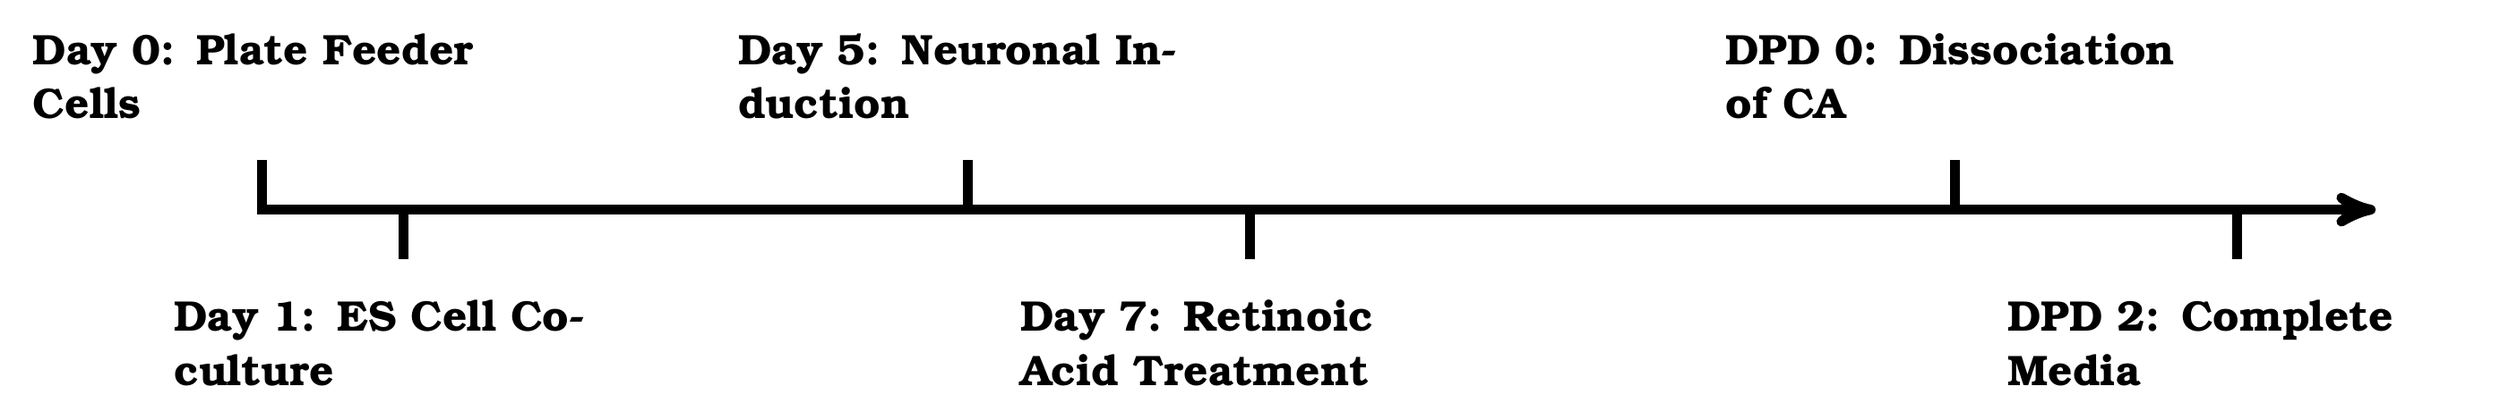
\begin{tikzpicture}[topline/.style={above=3pt,yshift=30pt,text width=6.5cm,font={\LARGE \bfseries}},
        bottomline/.style={below=3pt,yshift=-30pt,text width=6.5cm,font={\LARGE \bfseries}}]
      %draw horizontal line
      \draw[->,shorten >=1pt,>=stealth',line width=4pt] (-0.07,0) -- (30,0);
      %draw vertical lines
      \foreach \x in {0, 10, 24}{
        \draw[line width=4pt] (\x, 20pt) -- (\x,0pt);
      }
      \foreach \x in {2, 14, 28}{
        \draw[line width=4pt] (\x,-20pt) -- (\x,0pt);
      }
      %draw nodes
      \draw (0,0)  node[topline]    {Day 0: Plate Feeder Cells };
      \draw (2,0)  node[bottomline] {Day 1: ES Cell Co-culture};
      \draw (10,0) node[topline]    {Day 5: Neuronal Induction };
      \draw (14,0) node[bottomline] {Day 7: Retinoic Acid Treatment };
      \draw (24,0) node[topline]    {DPD 0: Dissociation of CA };
      \draw (28,0) node[bottomline] {DPD 2: Complete Media };
    \end{tikzpicture}
  }

  \begin{block}{\textbf{Figure 4.2}}
    Timeline for the differentiation of ES cells into neurons.
  \end{block}
\end{frame}

\begin{frame}
  \resizebox{\linewidth}{!}{
    \begin{tikzpicture}[every label/.style={font=\bfseries}, pic/.style={inner sep=0pt}]
      \node[pic] (nestin) [label={below:Nestin}]                                {\includegraphics[width=0.25\textwidth]{figures/nestin.pdf}};
      \node[pic] (map2)   [right=0.5mm of nestin,label={below:Map2}]            {\includegraphics[width=0.25\textwidth]{figures/map2.pdf}};
      \node[pic] (dcx)    [right=0.5mm of map2,label={below:Doublecortin}]      {\includegraphics[width=0.25\textwidth]{figures/dcx.pdf}};
      \node[pic] (bTub)   [right=0.5mm of dcx,label={below:$\beta$Tubulin III}] {\includegraphics[width=0.25\textwidth]{figures/betaTubulin.pdf}};
    \end{tikzpicture}
  }

  \begin{block}{\textbf{Figure 4.3}}
    High-throughput screening immunofluorescence characterization of differentiated ES cells in 96-well format at day 12, 10x magnification.
  \end{block}
\end{frame}

\section{Mouse embryonic stem cell-derived neuron high-throughput drug screen assay for Angelman syndrome}

\begin{frame}
  \begin{columns}
    \column{0.5\textwidth}
    \resizebox{\textwidth}{3in}{
      \begin{tikzpicture}[every label/.style={font=\Large\bfseries},pic/.style={inner sep=0pt}]
        \node[pic] (off)   [label={above left:B}]                      {\includegraphics[width=0.38\textwidth]{figures/imprint-off2.pdf}};
        \node[pic] (on)    [right= of off,label={above left:C}]        {\includegraphics[width=0.38\textwidth]{figures/imprint-on2.pdf}};
        \node[pic] (empty) [above right=0.5mm of off]                  {};
        \node[pic]         [above=0.5mm of empty,label={above left:A}] {\includegraphics[width=0.75\textwidth]{figures/time-course2.pdf}};
      \end{tikzpicture}
    }

    \column{0.5\textwidth}
    \begin{block}{\textbf{Figure 5.1}}
      Topotecan induces reactivation of paternal \emph{Ube3a} allele in ES cell-derived neurons. \textbf{A)} Boxplots of time course analysis of imprinted neurons (N = 10). \textbf{B)} Boxplots of \emph{Ube3a$^{YFP}$} ES cell-derived neurons at 2 and 13 days post dissociation (DPD) demonstrating the imprinting of paternal \emph{Ube3a}. \textbf{C)} Boxplots of ES cell-derived neurons at 13 DPD with vehicle (water) or Topotecan (300 nM) treatment demonstrating the reactivation of paternal \emph{Ube3a}. N = 15 neurons.
    \end{block}
  \end{columns}
\end{frame}


\end{document}
